\documentclass[a4paper,12pt,openany,oneside]{book}
\usepackage[portuguese]{babel}
\usepackage[utf8]{inputenc}
%\usepackage[latin1]{inputenc}
\usepackage{indentfirst}
%\usepackage[T1]{fontenc}
\usepackage[final]{pdfpages}
\usepackage{lmodern}
\usepackage{epigraph}
\usepackage{hyperref}

\usepackage{lipsum}
\usepackage[usestackEOL]{stackengine}

%mudando o djabo do capitulo
%usando exemplo: https://pt.sharelatex.com/learn/Sections_and_chapters
\usepackage{titlesec}
 
\titleformat
{\chapter} % command
[display] % shape
{\bfseries\Large\itshape} % format
{Chapitre \ \thechapter} % label
{0.5ex} % sep
{
    \rule{\textwidth}{1pt}
    \vspace{1ex}
    \centering
} 


\setcounter{secnumdepth}{3}
% Pacotes ....................................................................................
\input{configs/pacotes.tex}

% Novos Comandos .....................................................................
\input{configs/comandos.tex}
%\citationmode{abbr}

% Inicia o texto
\begin{document}

% Paginas iniciais (sem numera��o)
\pagestyle{empty}

% P�gina de rosto (capa interna)
%
% ********** Pagina de Rosto
%

% titlepage gera paginas sem numeracao
\begin{titlepage}

\begin{center}

\small

% O comando @{} no ambiente tabular x é  para criar um novo delimitador
% entre colunas que não a barra vertical | que é normalmente utilizada.
% O delimitador desejado vai entre as chaves. No exemplo, não há nada,
% de modo que o delimitador é vazio. Este recurso está sendo usado para
% eliminar o espaço que geralmente existe entre as colunas
\begin{tabularx}{\linewidth}{ c X }
% A figura foi colocada dentro de um parbox para que fique verticalmente
% centralizada em relação ao resto da linha
\parbox[c]{7cm}{\includegraphics[width=\linewidth]{polytech_logo}} &
\begin{center}
\textsf{\textsc{Polytech Nice Sophia\\ Analyse Conception Object
}} 
\end{center}

\end{tabularx}


% O vfill � um espa�o vertical que assume a m�xima dimens�o poss�vel
% Os vfill's desta p�gina foram utilizados para que o texto ocupe
% toda a folha
\vfill

\LARGE

\textbf{Modélisation object (version 2)}

\vfill

\Large

\textbf{\href{mailto:gabicavalcantesilva@gmail.com}{CAVALCANTE DA SILVA Gabriela},\\
\href{mailto:cesar.colle@gmail.com }{COLLE César},\\\href{mailto:oliveira.raquel.lopes@gmail.com}LOPES DE OLIVEIRA,\\ \href{mailto:arnold.schweitzer@gmail.com}{SCHWEITZER Arnold}}

\vfill

\normalsize

Enseignant: Colette Michel

\vfill

\hfill
\parbox{0.5\linewidth}{\textbf{
A faire:} Diagranne UC (he haute niveau); Diagramme UC détailllés et Scéncarios Cockburn correspondant.}


\vfill

\large

%Data
Valbonne, FR, février 26

\end{center}

\end{titlepage}
  

%Espa�amento 1 1/2
\onehalfspacing  

\clearpage

% Paginas introdut�rias (com numera��o romana)
\frontmatter

%sResumo
\include{01_Introducao/resumo} 

% Lista de conte�do (sum�rio, gerado automaticamente)
%\addcontentsline{toc}{chapter}{Sumario}
%\renewcommand{\contentsname}{Sumário}
%\tableofcontents  
\begingroup
\let\cleardoublepage\clearpage
\renewcommand{\contentsname}{Plan}
\tableofcontents
\endgroup


% Lista de figuras (gerada automaticamente)
%\cleardoublepage 
%\addcontentsline{toc}{chapter}{Liste des Images}  
%\listoffigures  


% P�ginas do texto principal (com cabe�alho)
\mainmatter
\pagestyle{headings}

% Para facilitar a organiza��o, foi criado um diret�rio para cada
% cap�tulo do documento, pois assim os arquivos das figuras ficam
% classificados por cap�tulos
% Introdu��o

%\mychapter{Introduction}
%\mychapterstar{Introduction}
\chapter{Introduction}
\label{Cap:introduction}
Nous avons décidé ici même de modéliser le comportement d’un péage d’autoroute.\\
La modélisation sera effectuée en UML et comportera en premier temps de la réécriture des demandes de la société d’autoroute, puis de détailler les activités liées a ce péage et finalement la modélisation objet permettant une implémentation future du logiciel souhaité par la société . La modélisation UML nous permettra de mieux cerner les attentes du client sur le logiciel qu’il souhaite utiliser pour la gestion de ses voies.
 

% Desenvolvimento
%

\mychapter{Réécriture}
\label{Cap:TD1}


\section{Description physique}
Nous avons perçu que le système demandé sur la gestion d’une voie de péage d’autoroute.
%Nous avons élaborré dans ce document une première description de système d’un péage d’autoroute.

\begin{figure}[h]
    \centering
    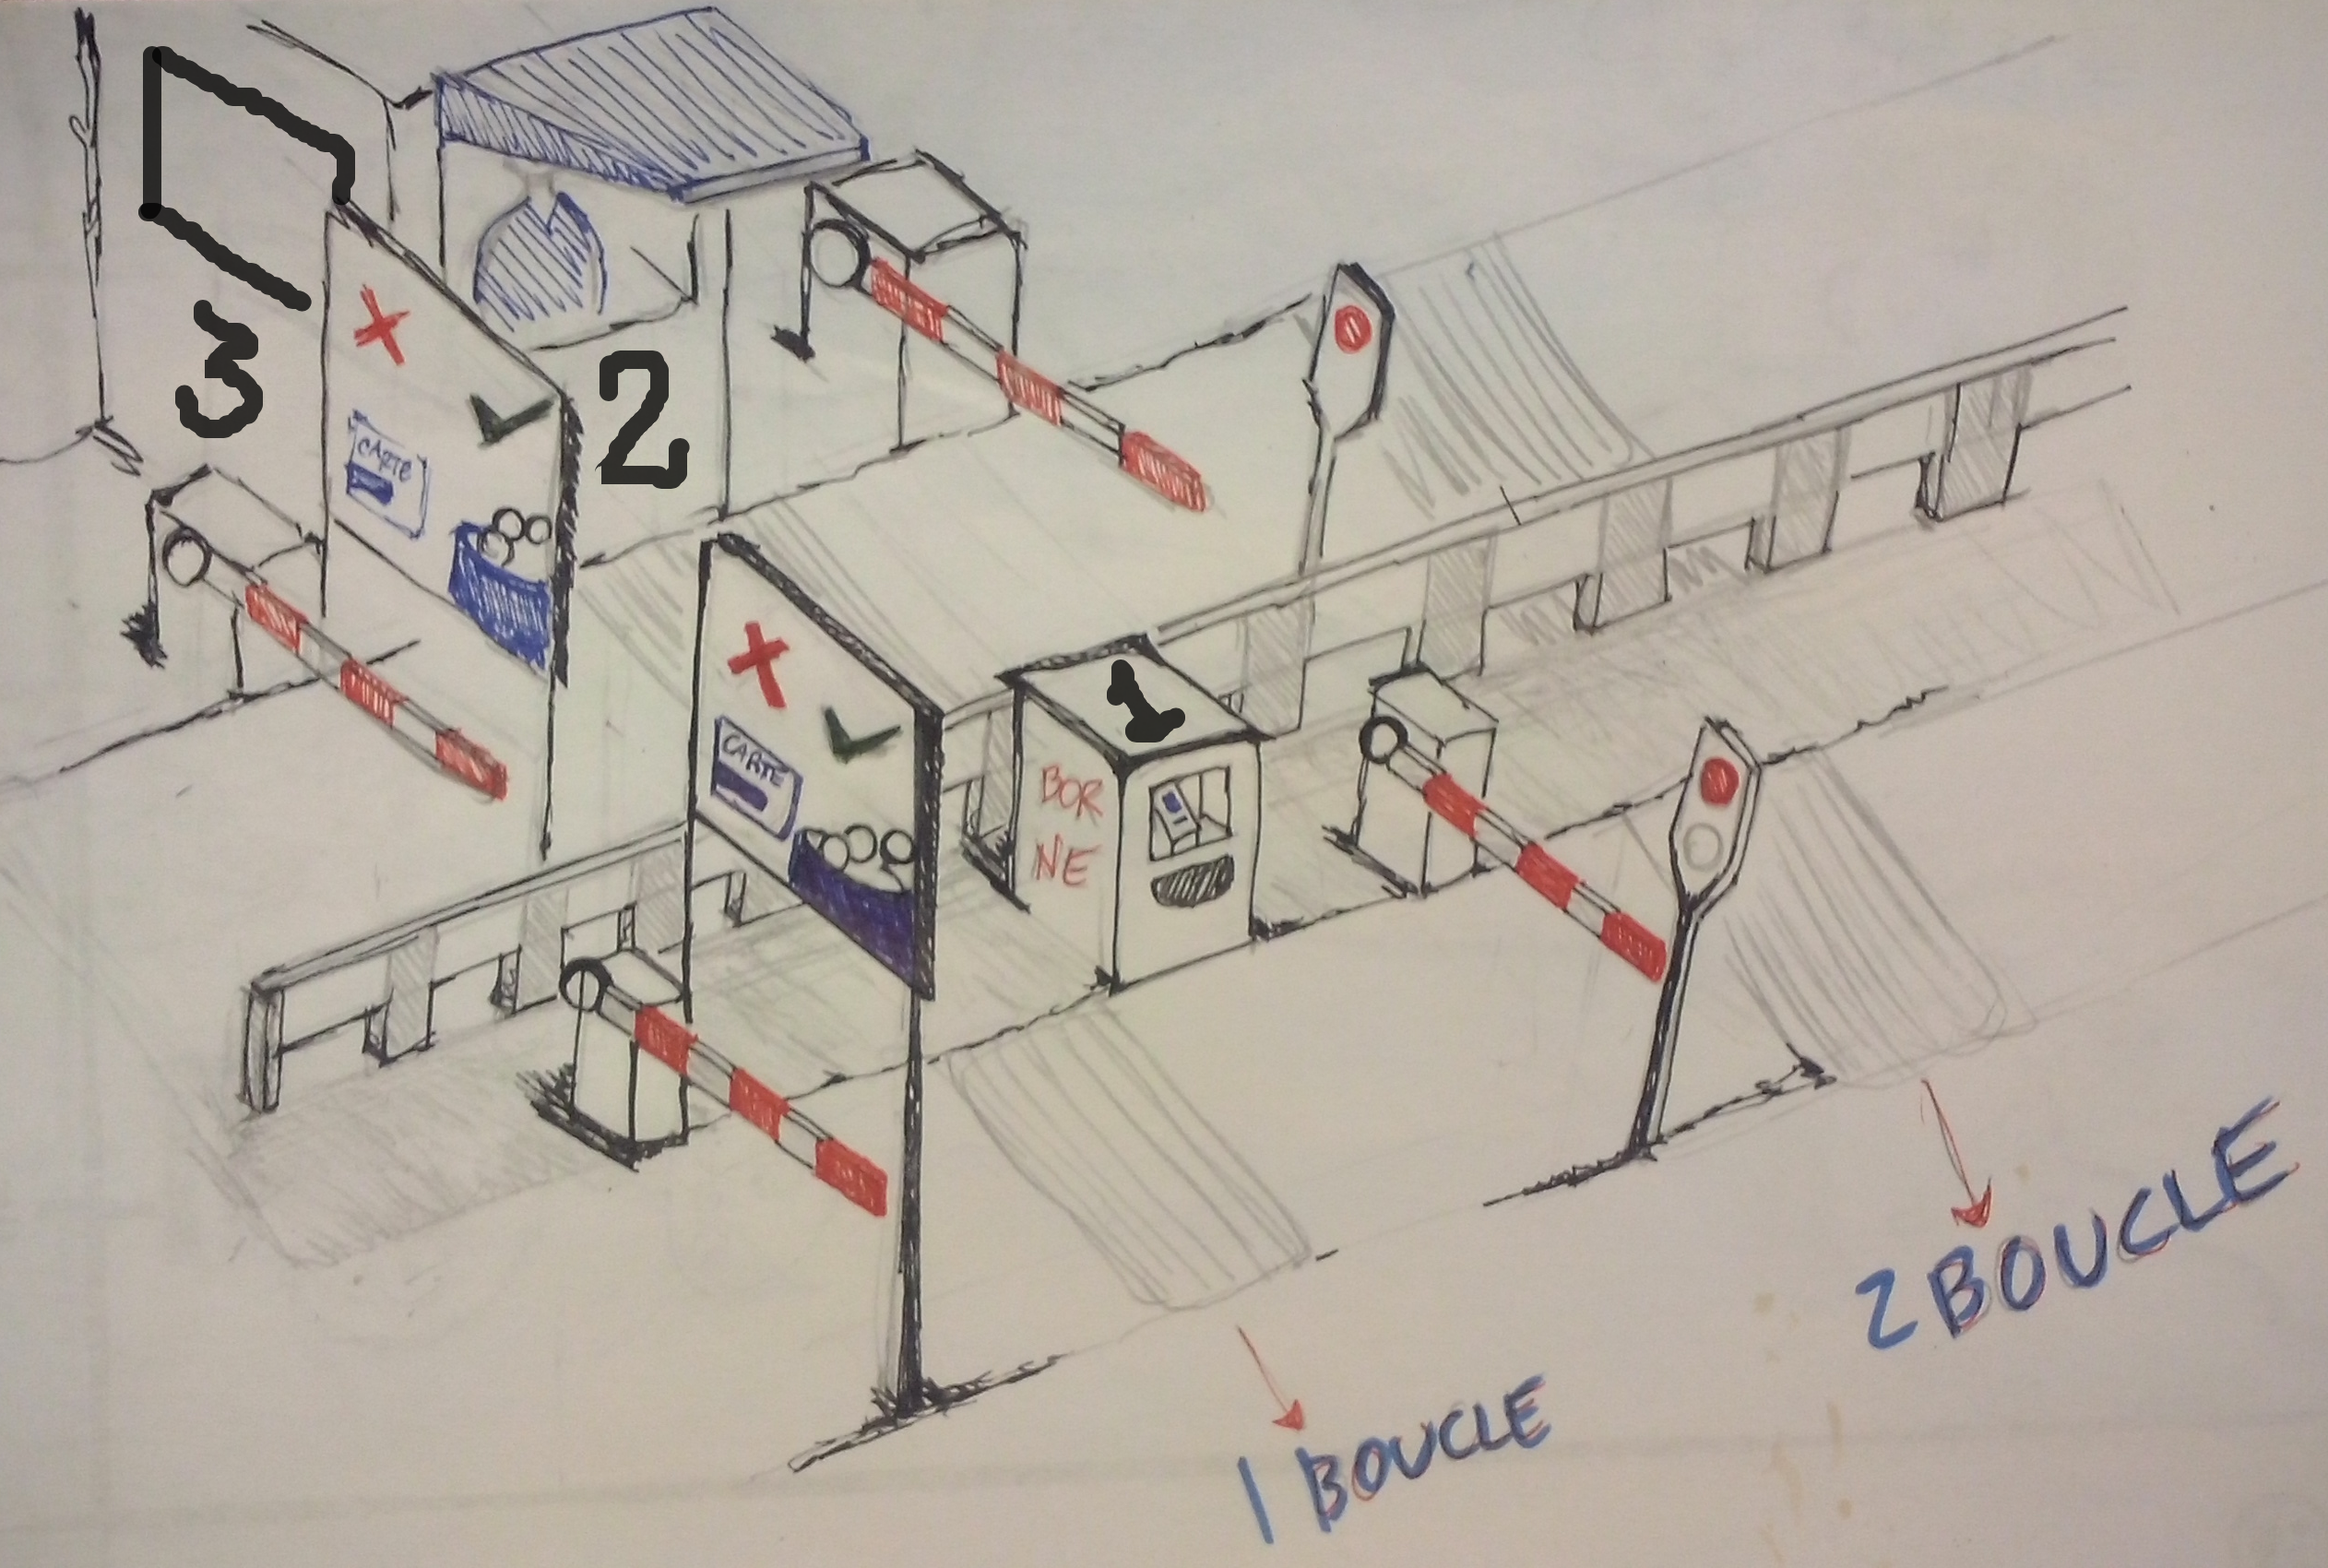
\includegraphics[scale=0.16]{02_Desenvolvimento/TD1/images/desc.png}
    \caption{Description physique}
    \label{fig:my_label}
\end{figure}
\newpage
\section{Réécriture de l'expression des besoins recentrée sur les utilisateurs du systeme}
\subsection{Les acteurs} 
Nous avons reconnu cinq acteurs (utilisateurs) du système tel que :
\begin{itemize}
    \item \textbf{Le Client (Conducteur de voiture)}: Le conducteur est le client, le rôle du conducteur est de passer la barrière de péage autoroutiere. 
    \item \textbf{La Société d’Autoroute}: 	La société est la propriétaire de la barrière de péage et gère donc la barrière. C’est elle qui va gérer aussi les cartes d’abonnement et le traitement des comptes des abonnés. 
    \item \textbf{Le Technicien}: Le technicien est l’acteur premier pour la maintenance du système. Le technicien lève la barrière manuellement en cas d’urgence. Il va faire des interventions humaines si necessaire, ex: si la barrière ne s’ouvre pas. 
    \item \textbf{Operateur humain}: L’ operateur humain reçoit le paiement du client (conducteur) dans les bornes manuelles.
    \item \textbf{Le Surveillant}: Les surveillants supervisent l’ensemble des bornes pour assurer, par exemple, qu’à tout moment il y ait une voie ouverte ou que le nombre de voies ouvertes soit proportionnel au flux de véhicules. Si le système lève une alarme vers l’ordinateur du poste de surveillance, un surveillant doit faire une intervention, comme remettre de la monnaie dans une borne et fait un compte-rendu approximatif de l’incident.
\end{itemize}
\newpage
\subsection{Les Grandes Fonctionnalités du Système}
Nous avons différencié trois grandes fonctionnalités du système:\\

\textbf{Passer le péage }(\ref{subsubsec:passerL})

\textbf{Gerer la comptapilité } (\ref{subsubsec:gerer})

\textbf{Maintenance }(\ref{subsubsec:maint})\\

Ainsi voici les scénarios informels correspondant :
\subsubsection{\textbf{Cas d’utilisation:} Passer le péage } \label{subsubsec:passerL} 
\textbf{Acteur primaire}: Le Client (le conducteur) 

\textbf{Acteur support}: La Société d’Autoroute, le technicien, l’operateur humain et le surveillant

Le client (le conducteur) opte pour une voie selon son type de véhicule et le moyen de paiement. Le client effectue le paiement selon le type de borne qu’ il a choisi (avec une carte d’abonnement, carte de crédit, monnaie, monnaie avec un opérateur humain, etc). Le système gère l’ouverture de la barrière une fois le montant payé ou la carte d’abonnement présenté, si la barrière ne s’ouvre pas, alors un technicien ou un opérateur doit venir régler l’incident survenu.


\subsubsection{\textbf{Cas d’utilisation:} Gerer la comptabilité}  \label{subsubsec:gerer}
\textbf{Acteur primaire}: La Société d'autoroute 

Le système doit assurer la comptabilité générale de l’ensemble des bornes. Chaque levée de barrière est enregistré. Les cartes d’abonnement et les compte des abonnés sont gérés par la société d’autoroute de façon instantanée, chaque passage est enregistré. Les opérations par cartes bleues sont gérées en fin de journée. Les bornes détectent les fausses pièces et les cartes volées.

\subsubsection{\textbf{Cas d’utilisation:} Maintenance}  \label{subsubsec:maint}
\textbf{Acteur primaire}: Le Technicien 

\textbf{Acteur support}: Le surveillant, l’opérateur humain

Le technicien permet de gérer toutes les cas, incidents, qui nécessitent une intervention humaine, lorsque qu’une barrière doit être ouverte ou fermée manuellement, lorsqu’un usager se retrouve coincé à la barrière de péage ou lorsqu’une borne a besoin de réglage ou de réparation (comme remettre de la monnaie).



\mychapter{Définitions de besoins}
\label{Cap:TD2}

\section{Diagramme UC de haut niveau - Péage}
    \begin{figure}[h]
    \centering
    \includegraphics[scale=0.50]{02_Desenvolvimento/TD2/images/hautNiveau.png}
    \caption{Diagramme de haut niveau - Péage}
    \label{fig:hautNiveau}
\end{figure}

\textbf{Scénario Informel:} Passer le péage\\
Le client (le conducteur) opte pour une voie d’autoroute selon son type de véhicule et le moyen de paiement. La borne détecte et valide le véhicule. Le conducteur effectue le paiement selon le type de borne qu’il a choisi (avec une carte d’abonnement, carte de crédit, monnaie, monnaie à un opérateur humain, etc). Le système gère l’ouverture de la barrière une fois le montant payé ou la carte d’abonnement présenté. Si la barrière ne s’ouvre pas ou si la borne détecte un véhicule non autorisé, alors un technicien ou un opérateur doit venir régler l’incident survenu. Si une borne automatique n'a plus de mannaie, donc il faut lever une alarme vers l'ordinateur du poste de surveillance. C'est le même traitement le déclenchement des mouvements de barrières, des affichages des panneaux indicatifs de l'ouverture au de la fermeture de la voie, la sychronisation feu et aval, etc.

\textbf{Scénario Informel:} Gerer la comptabilité \\
Le système doit assurer la comptabilité générale de l’ensemble des bornes. Chaque levée de barrière est enregistré. Les cartes d’abonnement et les compte des abonnés sont gérés par la société d’autoroute de façon instantanée, chaque passage est enregistré. Les opérations par cartes bleues sont gérées en fin de journée. Les bornes détectent les fausses pièces et les cartes volées.

\textbf{Scénario Informel:} Maintenance  \\
Le technicien permet de gérer toutes les cas, incidents, qui nécessitent une intervention humaine, lorsque qu’une barrière doit être ouverte ou fermée manuellement, lorsqu’un usager se retrouve coincé à la barrière de péage ou lorsqu’une borne a besoin de réglage ou de réparation (comme remettre de la monnaie).

\newpage
\section{Passer le péage}\label{sec:passer}
    \textbf{Cas d'utilisation:} Passer le péage
    
\textbf{Acteur primaire (initiateur):} Conducteur
    
%\textbf{Acteur support:} -

\textbf{Pré-condition: } Nécessite que la voie soit ouverte et libre

    
\textbf{Post-condition: }   La voie redevient disponible(ouverte et libre) pour un prochain usager.
    
\textbf{Scénario primaire: } \\
\textbf{1.} Le conducteur rentre dans la voie d’autoroute.(\ref{subsec:rentre})
 \\
\textbf{2.} Le conducteur paie le passage. (\ref{subsec:paie})\\
\textbf{3.} Le conducteur sort. (\ref{subsec:sortir})\\
    
\textbf{Variantes}\\
\textbf{1a.} Le conducteur n’arrive pas a rentrer dans la voie, dépannage et fin du scénario.\\
\textbf{3a.} le conducteur ne sort pas : la barrière reste fermer en attendant la sortie de conducteur.\\

\textbf{Décomposition des cas d'utilisation:} 
\begin{figure}[h]
    \centering
    \includegraphics[scale=0.7]{02_Desenvolvimento/TD2/images/passerLePassage.png}
    \caption{Décomposition des cas d'utilisation: Passer le péage}
\end{figure}


\newpage

\subsection{Rentrer} \label{subsec:rentre}
    \subsubsection{Scénario Cockburn}
\textbf{Cas d'utilisation: }Rentrer

\textbf{Acteur primaire:} Le conducteur

\textbf{Pré-condition: } La voie est libre et ouvertre.
 
\textbf{Post-condition: } Le systeme de paiement est opérationnel


\textbf{Scénario primaire: } \\
    \textbf{1.} La boucle détecte le véhicule.\\
    \textbf{2.} La boucle envoi l’information à la borne.\\
    \textbf{3.} La borne détermine le type de véhicule. Le type est autorisé. \\
    \textbf{4.} La borne affiche le montant sur l'écran.\\

\textbf{Variantes:}\\
    \textbf{1a.} La boucle ne repère pas le véhicule, l’utilisateur ne peut pas passer. L’utilisateur doit appeler le technicien. Fin scénario.\\
    \textbf{3a.}L’opérateur repère un véhicule prioritaire en urgence. L’opérateur ouvre la barrière manuellement. Fin scénario. \\
    \textbf{3b.} Le type de véhicule n’est pas autorisé. Le conducteur appelle le technicien.\\
    \textbf{4a.} La borne n’affiche pas le montant, l’utilisateur ne peut pas payer , le conducteur appelle le technicien.\\
\newpage    
\subsubsection{Diagramme d'activité}
\begin{figure}[!htb]
    \centering
    \includegraphics[scale=0.45, angle = 90]{02_Desenvolvimento/TD2/images/DARentrer.png}
    \caption{Diagramme d'activité - Rentrer}
    \label{fig:DARentrer}
\end{figure}
\newpage
\subsubsection{Collaboration}
\begin{figure}[!htb]
    \centering
    \includegraphics[scale=0.7]{02_Desenvolvimento/TD2/images/ColaRentrer.png}
    \caption{Collaboration - Rentrer}
    \label{fig:DARentrer}
\end{figure}
\newpage
\subsubsection{Diagramme de séquence ( à revisiter )}
\begin{figure}[!htb]
    \centering
    \includegraphics[scale=0.5]{02_Desenvolvimento/TD2/images/DSRentrer.png}
    \caption{Diagramme de séquence à revisiter  - Rentrer}
    \label{fig:DARentrer}
\end{figure}
\subsubsection{Diagramme de séquence}
\begin{figure}[!htb]
    \centering
    \includegraphics[scale=0.5]{02_Desenvolvimento/TD2/images/v2-DSRentrer.png}
    \caption{Diagramme de séquence - Rentrer}
    \label{fig:DARentrer}
\end{figure}

\newpage

\subsection{Payer le passage} \label{subsec:paie}
    \subsubsection{Scénario Cockburn}
\textbf{Cas d'utilisation:} Payer le passage

\textbf{Acteur primaire:} Conducteur

\textbf{Acteur support:} Le poste de surveillance et opérateur humain (si le borne est manuelle)

\textbf{Pré-condition: }  la borne est opérationnelle

\textbf{Post-condition: }  la transaction(paiement) est acceptée.

\textbf{Scenario primaire: } \\ 
    \textbf{1.} Le conducteur paye en liquide %(\ref{subsec:paieLiquide}) 
    \\ 
    \textbf{2.} La transaction est enregistrée dans l’ordinateur central de la société d’autoroute.\\ 

\textbf{Variantes:}\\
    \textbf{1a.} Le conduteur paye par carte
    \\
    \textbf{1b.} Le conducteur paye par télépéage.
     \\
    \textbf{1d.} la transaction(paiement) a échoué. Retourne à l’état 1. \\ %he clicks in the botton who calls the technicien 
\newpage
\subsubsection{Décomposition de cas d'utilisation (Généralisation):} 
\begin{figure}[h]
    \centering
    \includegraphics[scale=0.5]{02_Desenvolvimento/TD2/images/PayeGeneralisation.png}
    \caption{Généralisation de cas d'utilisation: Payer le passage}
\end{figure}
\subsubsection{Collaboration}
\begin{figure}[h]
    \centering
    \includegraphics[scale=0.6]{02_Desenvolvimento/TD2/images/ColaPayer.png}
    \caption{Diagramme d'activité: Payer le passage}
\end{figure}
\newpage
\subsubsection{Diagramme d'activité}
\begin{figure}[h]
    \centering
    \includegraphics[scale=0.6]{02_Desenvolvimento/TD2/images/DAPayePassage.png}
    \caption{Diagramme d'activité: Payer le passage}
\end{figure}

 
 \newpage   
\subsection{Payer en liquide} \label{subsec:paieLiquide}
    \subsection{Scénario Cockburn}
\textbf{Cas d'utilisation:} Payer en liquide

\textbf{Acteur primaire:} Le Conducteur

\textbf{Pré-condition: } la borne affiche le montant
 

\textbf{Scénario primaire: } \\
    \textbf{1.} Le conducteur insère de l’argent liquide.\\
    \textbf{2.}  La borne enclenche la détection de fausse pièce. La borne valide les pièces.\\
    \textbf{3.} La borne analyse le montant . Le conducteur a donné le montant exact.\\
    \textbf{4.} La borne accepte le paiement.

\textbf{Variantes:}\\
    \textbf{2a.} La borne ne valide pas les pièces . La borne rend les pièces invalides.\\
    \textbf{3a.} La borne analyse le montant . Le conducteur donne un montant plus grand que celui de la borne. La borne rend la différence entre la somme introduite et le montant demandé.\\
    \textbf{3b.} La borne analyse le montant . Le conducteur donne un montant moins que celui de la borne. Se met en attente.\\
    \textbf{4a.} Le borne n’accepte pas le paiement. Appelle le technicien. \\
    \textbf{3a1.} La borne n’a plus de monnaie, la borne emet un signal pour avertir le technicien
\\
    
\newpage
\subsection{Diagramme d'activité}
\begin{figure}[h]
    \centering
    \includegraphics[scale=0.45]{02_Desenvolvimento/TD2/images/DAPayeLiquide.png}
    \caption{Diagramme d'activité: Payer en liquide}
\end{figure}
\newpage
\subsection{Collaboration}
\begin{figure}[h]
    \centering
    \includegraphics[scale=0.55]{02_Desenvolvimento/TD2/images/ColaLiquide.png}
    \caption{Collaboration: Payer en liquide}
\end{figure}
\newpage   
\subsection{Payer par carte} 
    \subsubsection{Scénario Cockburn}
\textbf{Cas d'utilisation:} Payer par carte

\textbf{Acteur primaire:} Le conducteur

\textbf{Pré-condition: } La borne accepte le payement par carte.
 
\textbf{Post-condition: }  La transaction a été acceptée ou pas.

\textbf{Scenario primaire: } \\
    \textbf{1.} Le conducteur insère sa carte. \\
    \textbf{2.} Le lecteur détecte une carte bleue. \\
    \textbf{3.} Le lecteur effectue un paiement par carte bleue.\\
    \textbf{4.} Le conducteur récupère sa carte.\\

\textbf{Variantes:}\\
    \textbf{2a1.} Le lecteur détecte une carte d’abonnement.\\
    \textbf{2a2.} Le lecteur effectue un paiement par abonnement. Aller en 4.\\
    \textbf{2b.} Le lecteur détecte une carte non valide.  Aller en 4. \\
    
\newpage
\subsubsection{Diagramme d'activité}
\begin{figure}[h]
    \centering
    \includegraphics[scale=0.45]{02_Desenvolvimento/TD2/images/DA-PayerCarte.png}
    \caption{Diagramme d'activité: Payer par carte}
\end{figure}
\newpage
\subsubsection{Collaboration}
\begin{figure}[h]
    \centering
    \includegraphics[scale=0.6]{02_Desenvolvimento/TD2/images/ColaCarte.png}
    \caption{Collaboration: Payer par carte}
\end{figure}
    
    
\newpage
\subsection{Payer par carte bleue} \label{subsec:paierBleu}
    \subsubsection{Scénario Cockburn}
\textbf{Cas d'utilisation:} Payer par carte bleue

\textbf{Acteur primaire:} Le conducteur

\textbf{Pré-condition: } Le conducteur insère sa carte bleue dans la borne.

\textbf{Post-condition: }  La transaction a été validé ou pas.


\textbf{Scénario primaire: } \\
    \textbf{1.} Le lecteur de carte analyse la  carte bleue : la carte n’est pas une carte volée.\\ 
    \textbf{2.} La borne accepte le transaction(paiement). \\
  
\textbf{Variantes:}\\
    \textbf{1a1.} La vérification auprès des cartes volées indique que la carte bleue est volée.\\
    \textbf{1a2.} La transaction est échoue(payement est refusé). Fin scénario.\\
    
\newpage
\subsubsection{Diagramme d'activité}
\begin{figure}[h]
    \centering
    \includegraphics[scale=0.8]{02_Desenvolvimento/TD2/images/DAPayeBleu.png}
    \caption{Diagramme d'activité: Payer par carte bleue}
\end{figure}
\newpage
\subsubsection{Collaboration}
\begin{figure}[h]
    \centering
    \includegraphics[scale=0.6]{02_Desenvolvimento/TD2/images/ColaCarteBleu.png}
    \caption{Collaboration: Payer par carte bleue}
\end{figure}
\newpage    
\subsubsection{Diagramme de séquence}
\begin{figure}[!htb]
    \centering
    \includegraphics[scale=0.5]{02_Desenvolvimento/TD2/images/DS-payerCarteBleu.png}
    \caption{Diagramme de séquence - Payer par carte bleue - à revisiter }
\end{figure}
\subsubsection{Diagramme de séquence}
\begin{figure}[!htb]
    \centering
    \includegraphics[scale=0.5]{02_Desenvolvimento/TD2/images/v2-DS-payerCarteBleu.png}
    \caption{Diagramme de séquence - Payer par carte bleue}
\end{figure}
\newpage

\subsection{Payer par carte d'abonnement} \label{subsec:paierAbonement}
    \subsubsection{Scénario Cockburn}
\textbf{Cas d'utilisation:} Payer par carte d'abonnement

\textbf{Acteur primaire:} Le conducteur

\textbf{Pré-condition: }  La borne affiche le montant.

 
\textbf{Post-condition: }  La transaction(payement) a été validé ou pas.

\textbf{Scenario primaire: } \\
    \textbf{1.} Le lecteur vérifie la carte d'abonnement. La carte est valide. \\
    \textbf{2.} La borne accepte le payement.\\

\textbf{Variantes:}\\
    \textbf{1a1.}   Le lecteur détecte une carte d'abonnement invalide.\\
    \textbf{1a2.}   La transaction est échoue(payement est refusé). Fin scénario.\\
    
\newpage
\subsubsection{Diagramme d'activité}
\begin{figure}[h]
    \centering
    \includegraphics[scale=0.6]{02_Desenvolvimento/TD2/images/DAAbonnement.png}
    \caption{Diagramme d'activité: Payer par carte d'abonnement}
\end{figure}
\newpage
\subsubsection{Collaboration}
\begin{figure}[h]
    \centering
    \includegraphics[scale=0.6]{02_Desenvolvimento/TD2/images/ColaCarteAbonnement.png}
    \caption{Collaboration: Payer par carte d'abonnement}
\end{figure}
\newpage    
\subsubsection{Diagramme de séquence}
\begin{figure}[!htb]
    \centering
    \includegraphics[scale=0.5]{02_Desenvolvimento/TD2/images/DS-payerAbonnement.png}
    \caption{Diagramme de séquence - Payer par carte d'abonnement - à revisiter }
\end{figure}
\subsubsection{Diagramme de séquence}
\begin{figure}[!htb]
    \centering
    \includegraphics[scale=0.5]{02_Desenvolvimento/TD2/images/v2-DS-payerCarteAbonnement.png}
    \caption{Diagramme de séquence - Payer par carte d'abonnement}
\end{figure}
    
\newpage  
\subsection{Payer par télépéage} \label{subsec:paierTelepeage}
    \subsection{Scénario Cockburn}
\textbf{Cas d'utilisation: Payer par Télépéage}

\textbf{Acteur primaire:} Le conducteur

%\textbf{Acteur support:}

\textbf{Pré-condition: }  La borne est une borne télépéage ou mixte
 
%\textbf{Post-condition: } 

\textbf{Scenario primaire: } \\
    \textbf{1.} La borne détecte le badge télépéage\\
    \textbf{2.} La borne enregistre le passage dans l’ordinateur central.\\

\textbf{Variantes:}\\
    \textbf{1a.} La borne ne détecte pas le badge. un technicien est appellé.\\
   \textbf{2a.} La borne n’ouvre pas la barrière. Le conducteur appelle le technicien.\\



%\subsection{{Décomposition des cas d'utilisation:} 
%\begin{figure}[h]
 %   \centering
  %  \includegraphics[scale=0.7]{02_Desenvolvimento/TD2/images/PaiementTelepeage.png}
   % \caption{Décomposition des cas d'utilisation: Payer avec abonnement Télépéage}
%\end{figure}
\newpage
\subsection{Diagramme d'activité}
\begin{figure}[h]
    \centering
    \includegraphics[scale=0.7]{02_Desenvolvimento/TD2/images/DATelepeage.png}
    \caption{Diagramme d'activité: Payer par Telépéage}
\end{figure}
\newpage
\subsection{Collaboration}
\begin{figure}[h]
    \centering
    \includegraphics[scale=0.6]{02_Desenvolvimento/TD2/images/ColaTelepeage.png}
    \caption{Collaboration: Payer par Telépéage}
\end{figure}


\newpage    
\subsection{Sortir} \label{subsec:sortir}
%Scénario n'a pas été décrit.
    \subsubsection{Scénario Cockburn}
\textbf{Cas d'utilisation:} Sortir

\textbf{Acteur primaire:}  Le conducteur

\textbf{Pré-condition:} La transaction (paiement) a été accepté.

 
\textbf{Post-condition:} Le deuxième barriere est abaissée. 

\textbf{Scenario primaire: } \\
    \textbf{1.}  La borne change la couleur du feu (vert). \\
    \textbf{2.} La borne léve la deuxième barrière. \\
    \textbf{3.} Le conducteur se dirige vers la deuxième barrière.\\
    \textbf{4.} Le deuxième boucle detecte que le véhicule est sorti.\\ 
    \textbf{5.}  La borne change la couleur du feu (rouge).\\
    \textbf{6.}  La borne abaisse la deuxième barrière. \\

\textbf{Variantes:}\\
    \textbf{1a.} Le feu ne change pas de couleur. Donc une alarme est levé vers le technicien. Fin scénario.\\
    \textbf{2a.}  . La deuxième barriere barriere ne se léve pas. Donc une alarme est levé vers le technicien. Fin scenário.\\
    \textbf{4a.}  La boucle ne détecte pas que le véhicule est sortie. La barrière reste levée.Fin scénario.\\
\newpage    
\subsubsection{Diagramme d'activité}
\begin{figure}[!htb]
    \centering
    \includegraphics[scale=0.4, angle = 90]{02_Desenvolvimento/TD2/images/DASortir.png}
    \caption{Diagramme d'activité - Sortir}
    \label{fig:DARentrer}
\end{figure}
\newpage    
\subsubsection{Collaboration}
\begin{figure}[!htb]
    \centering
    \includegraphics[scale=0.6]{02_Desenvolvimento/TD2/images/ColaSortir.png}
    \caption{Collaboration - Sortir}
    \label{fig:DARentrer}
\end{figure}
\newpage    
\subsubsection{Diagramme de séquence}
\begin{figure}[!htb]
    \centering
    \includegraphics[scale=0.5]{02_Desenvolvimento/TD2/images/DSSortir.png}
    \caption{Diagramme de séquence - Sortir - à revisiter }
    \label{fig:DARentrer}
\end{figure}
\subsubsection{Diagramme de séquence}
\begin{figure}[!htb]
    \centering
    \includegraphics[scale=0.5]{02_Desenvolvimento/TD2/images/v2-DSSortir.png}
    \caption{Diagramme de séquence - Sortir}
    \label{fig:DARentrer}
\end{figure}

\newpage 


\mychapter{Réécriture}
\label{Cap:TD1}


\section{Description physique}
Nous avons perçu que le système demandé sur la gestion d’une voie de péage d’autoroute.
%Nous avons élaborré dans ce document une première description de système d’un péage d’autoroute.

\begin{figure}[h]
    \centering
    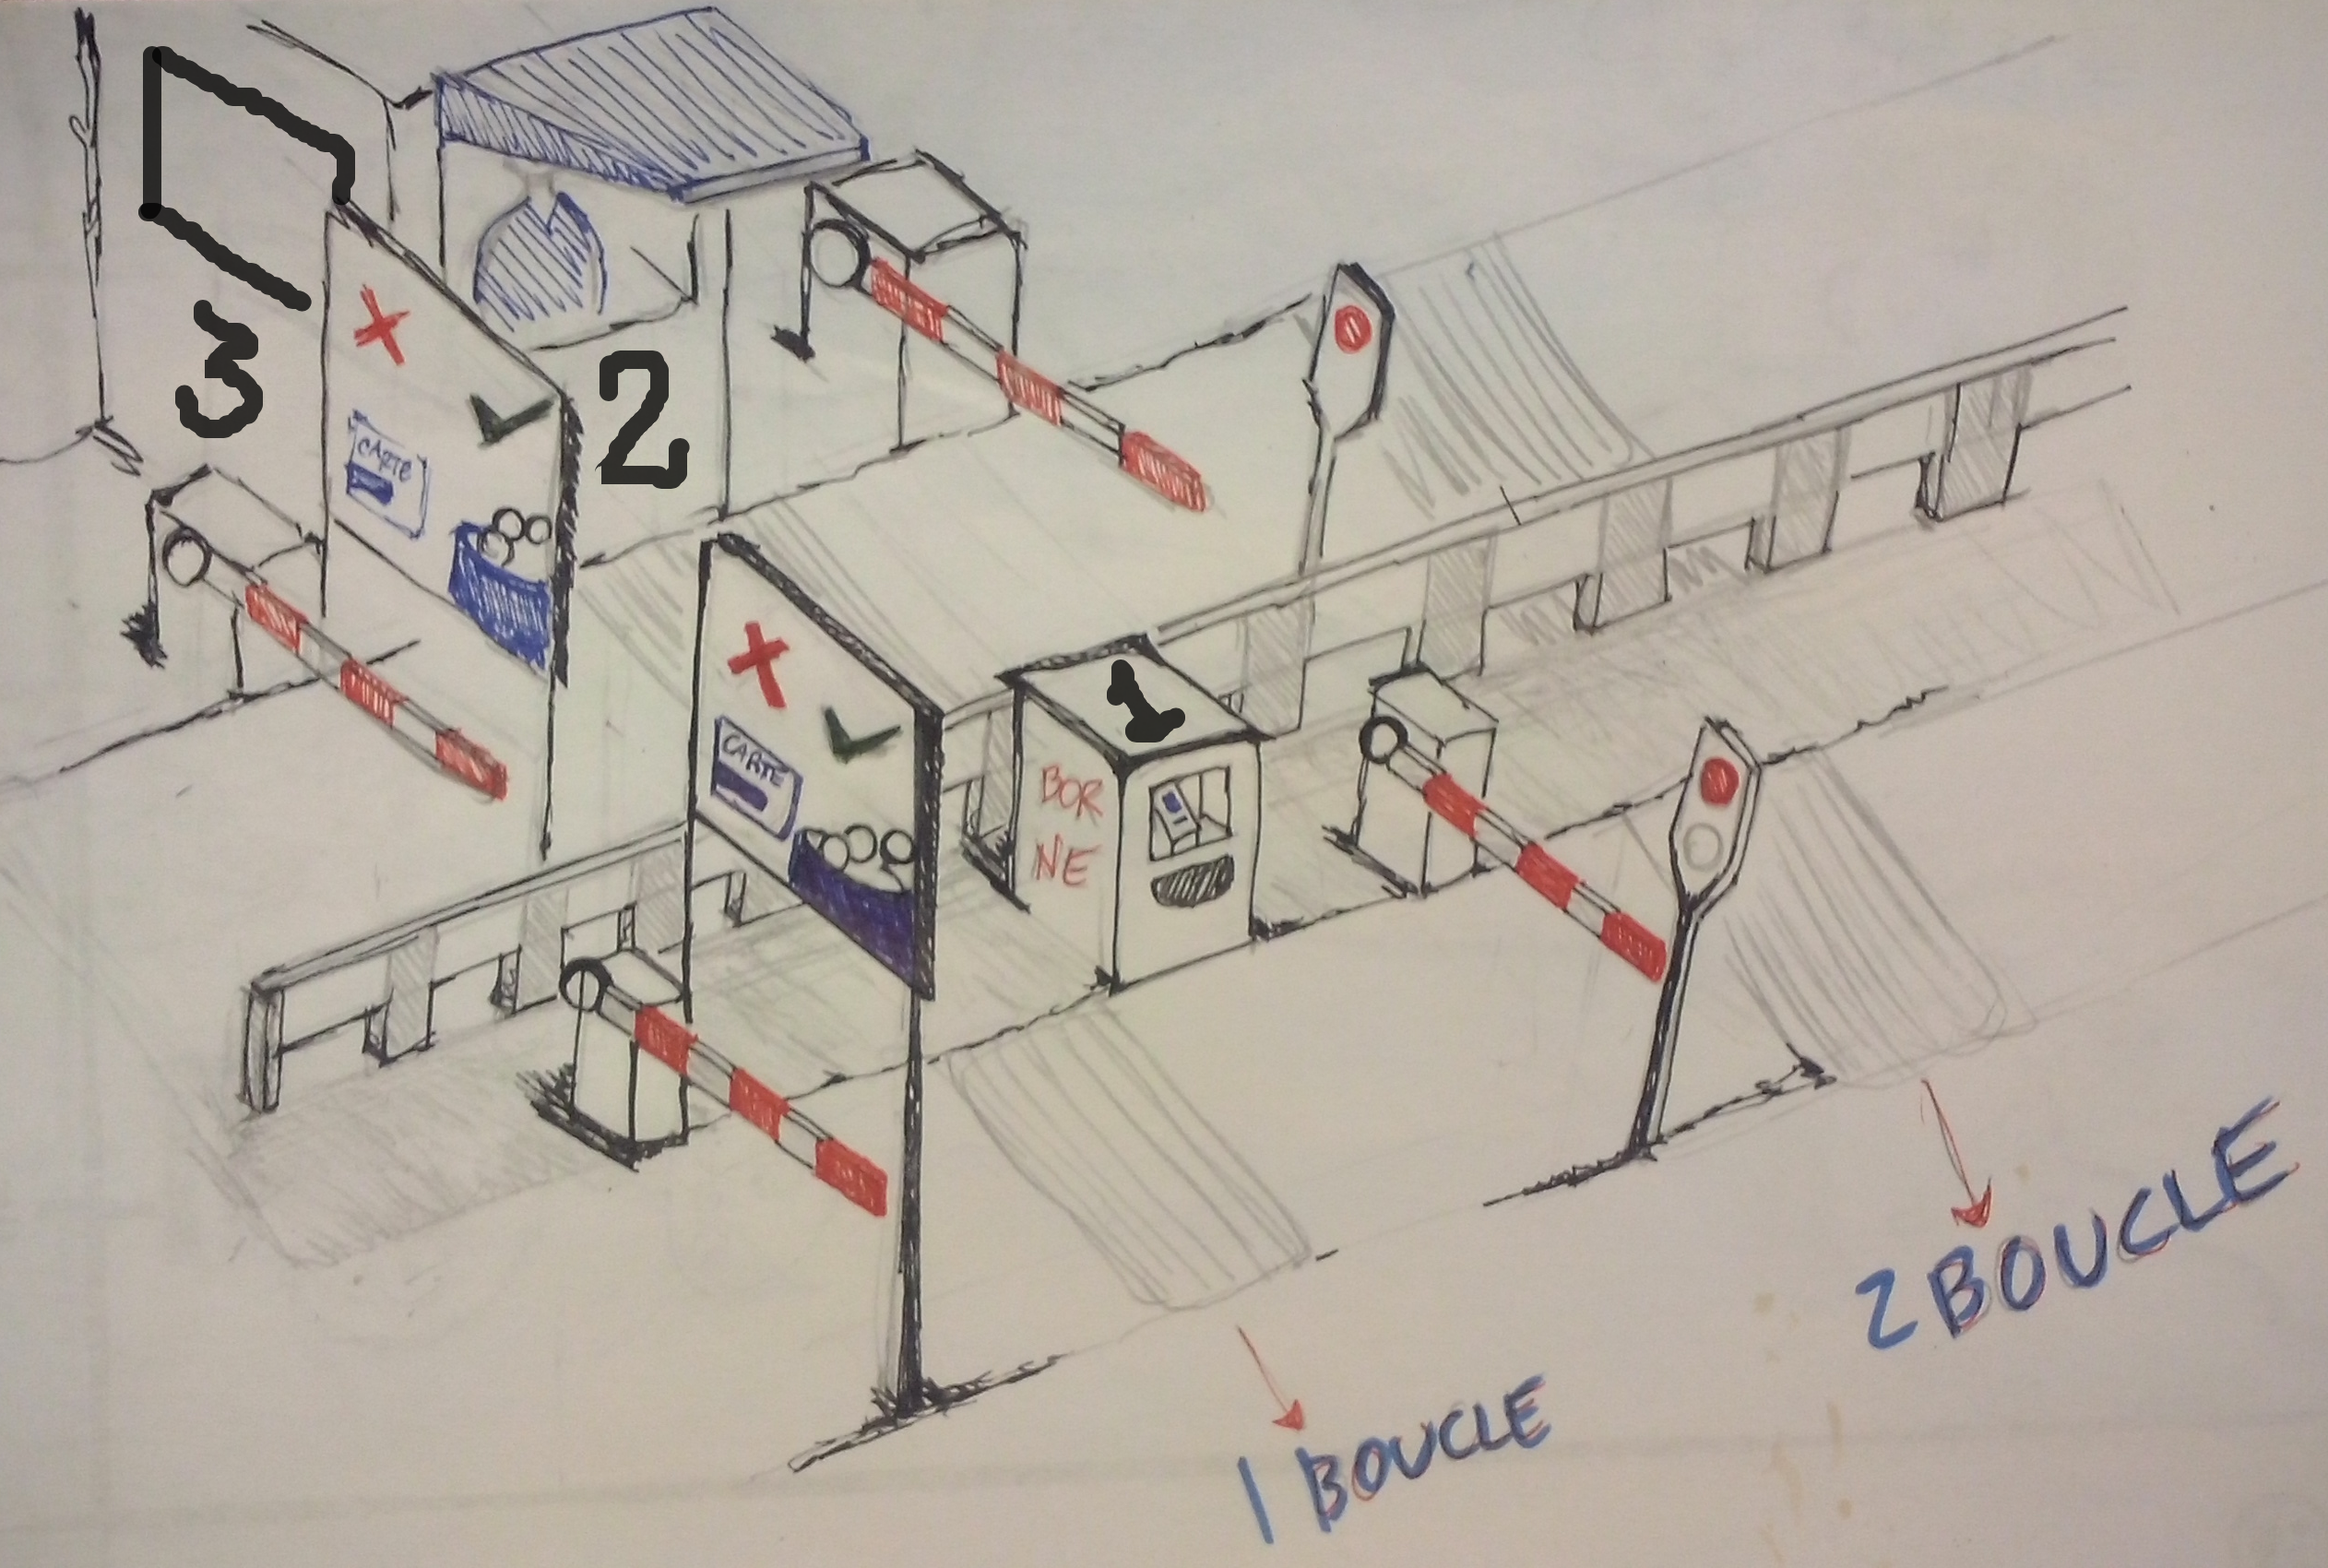
\includegraphics[scale=0.16]{02_Desenvolvimento/TD1/images/desc.png}
    \caption{Description physique}
    \label{fig:my_label}
\end{figure}
\newpage
\section{Réécriture de l'expression des besoins recentrée sur les utilisateurs du systeme}
\subsection{Les acteurs} 
Nous avons reconnu cinq acteurs (utilisateurs) du système tel que :
\begin{itemize}
    \item \textbf{Le Client (Conducteur de voiture)}: Le conducteur est le client, le rôle du conducteur est de passer la barrière de péage autoroutiere. 
    \item \textbf{La Société d’Autoroute}: 	La société est la propriétaire de la barrière de péage et gère donc la barrière. C’est elle qui va gérer aussi les cartes d’abonnement et le traitement des comptes des abonnés. 
    \item \textbf{Le Technicien}: Le technicien est l’acteur premier pour la maintenance du système. Le technicien lève la barrière manuellement en cas d’urgence. Il va faire des interventions humaines si necessaire, ex: si la barrière ne s’ouvre pas. 
    \item \textbf{Operateur humain}: L’ operateur humain reçoit le paiement du client (conducteur) dans les bornes manuelles.
    \item \textbf{Le Surveillant}: Les surveillants supervisent l’ensemble des bornes pour assurer, par exemple, qu’à tout moment il y ait une voie ouverte ou que le nombre de voies ouvertes soit proportionnel au flux de véhicules. Si le système lève une alarme vers l’ordinateur du poste de surveillance, un surveillant doit faire une intervention, comme remettre de la monnaie dans une borne et fait un compte-rendu approximatif de l’incident.
\end{itemize}
\newpage
\subsection{Les Grandes Fonctionnalités du Système}
Nous avons différencié trois grandes fonctionnalités du système:\\

\textbf{Passer le péage }(\ref{subsubsec:passerL})

\textbf{Gerer la comptapilité } (\ref{subsubsec:gerer})

\textbf{Maintenance }(\ref{subsubsec:maint})\\

Ainsi voici les scénarios informels correspondant :
\subsubsection{\textbf{Cas d’utilisation:} Passer le péage } \label{subsubsec:passerL} 
\textbf{Acteur primaire}: Le Client (le conducteur) 

\textbf{Acteur support}: La Société d’Autoroute, le technicien, l’operateur humain et le surveillant

Le client (le conducteur) opte pour une voie selon son type de véhicule et le moyen de paiement. Le client effectue le paiement selon le type de borne qu’ il a choisi (avec une carte d’abonnement, carte de crédit, monnaie, monnaie avec un opérateur humain, etc). Le système gère l’ouverture de la barrière une fois le montant payé ou la carte d’abonnement présenté, si la barrière ne s’ouvre pas, alors un technicien ou un opérateur doit venir régler l’incident survenu.


\subsubsection{\textbf{Cas d’utilisation:} Gerer la comptabilité}  \label{subsubsec:gerer}
\textbf{Acteur primaire}: La Société d'autoroute 

Le système doit assurer la comptabilité générale de l’ensemble des bornes. Chaque levée de barrière est enregistré. Les cartes d’abonnement et les compte des abonnés sont gérés par la société d’autoroute de façon instantanée, chaque passage est enregistré. Les opérations par cartes bleues sont gérées en fin de journée. Les bornes détectent les fausses pièces et les cartes volées.

\subsubsection{\textbf{Cas d’utilisation:} Maintenance}  \label{subsubsec:maint}
\textbf{Acteur primaire}: Le Technicien 

\textbf{Acteur support}: Le surveillant, l’opérateur humain

Le technicien permet de gérer toutes les cas, incidents, qui nécessitent une intervention humaine, lorsque qu’une barrière doit être ouverte ou fermée manuellement, lorsqu’un usager se retrouve coincé à la barrière de péage ou lorsqu’une borne a besoin de réglage ou de réparation (comme remettre de la monnaie).



\mychapter{Définitions de besoins}
\label{Cap:TD2}

\section{Diagramme UC de haut niveau - Péage}
    \begin{figure}[h]
    \centering
    \includegraphics[scale=0.50]{02_Desenvolvimento/TD2/images/hautNiveau.png}
    \caption{Diagramme de haut niveau - Péage}
    \label{fig:hautNiveau}
\end{figure}

\textbf{Scénario Informel:} Passer le péage\\
Le client (le conducteur) opte pour une voie d’autoroute selon son type de véhicule et le moyen de paiement. La borne détecte et valide le véhicule. Le conducteur effectue le paiement selon le type de borne qu’il a choisi (avec une carte d’abonnement, carte de crédit, monnaie, monnaie à un opérateur humain, etc). Le système gère l’ouverture de la barrière une fois le montant payé ou la carte d’abonnement présenté. Si la barrière ne s’ouvre pas ou si la borne détecte un véhicule non autorisé, alors un technicien ou un opérateur doit venir régler l’incident survenu. Si une borne automatique n'a plus de mannaie, donc il faut lever une alarme vers l'ordinateur du poste de surveillance. C'est le même traitement le déclenchement des mouvements de barrières, des affichages des panneaux indicatifs de l'ouverture au de la fermeture de la voie, la sychronisation feu et aval, etc.

\textbf{Scénario Informel:} Gerer la comptabilité \\
Le système doit assurer la comptabilité générale de l’ensemble des bornes. Chaque levée de barrière est enregistré. Les cartes d’abonnement et les compte des abonnés sont gérés par la société d’autoroute de façon instantanée, chaque passage est enregistré. Les opérations par cartes bleues sont gérées en fin de journée. Les bornes détectent les fausses pièces et les cartes volées.

\textbf{Scénario Informel:} Maintenance  \\
Le technicien permet de gérer toutes les cas, incidents, qui nécessitent une intervention humaine, lorsque qu’une barrière doit être ouverte ou fermée manuellement, lorsqu’un usager se retrouve coincé à la barrière de péage ou lorsqu’une borne a besoin de réglage ou de réparation (comme remettre de la monnaie).

\newpage
\section{Passer le péage}\label{sec:passer}
    \textbf{Cas d'utilisation:} Passer le péage
    
\textbf{Acteur primaire (initiateur):} Conducteur
    
%\textbf{Acteur support:} -

\textbf{Pré-condition: } Nécessite que la voie soit ouverte et libre

    
\textbf{Post-condition: }   La voie redevient disponible(ouverte et libre) pour un prochain usager.
    
\textbf{Scénario primaire: } \\
\textbf{1.} Le conducteur rentre dans la voie d’autoroute.(\ref{subsec:rentre})
 \\
\textbf{2.} Le conducteur paie le passage. (\ref{subsec:paie})\\
\textbf{3.} Le conducteur sort. (\ref{subsec:sortir})\\
    
\textbf{Variantes}\\
\textbf{1a.} Le conducteur n’arrive pas a rentrer dans la voie, dépannage et fin du scénario.\\
\textbf{3a.} le conducteur ne sort pas : la barrière reste fermer en attendant la sortie de conducteur.\\

\textbf{Décomposition des cas d'utilisation:} 
\begin{figure}[h]
    \centering
    \includegraphics[scale=0.7]{02_Desenvolvimento/TD2/images/passerLePassage.png}
    \caption{Décomposition des cas d'utilisation: Passer le péage}
\end{figure}


\newpage

\subsection{Rentrer} \label{subsec:rentre}
    \subsubsection{Scénario Cockburn}
\textbf{Cas d'utilisation: }Rentrer

\textbf{Acteur primaire:} Le conducteur

\textbf{Pré-condition: } La voie est libre et ouvertre.
 
\textbf{Post-condition: } Le systeme de paiement est opérationnel


\textbf{Scénario primaire: } \\
    \textbf{1.} La boucle détecte le véhicule.\\
    \textbf{2.} La boucle envoi l’information à la borne.\\
    \textbf{3.} La borne détermine le type de véhicule. Le type est autorisé. \\
    \textbf{4.} La borne affiche le montant sur l'écran.\\

\textbf{Variantes:}\\
    \textbf{1a.} La boucle ne repère pas le véhicule, l’utilisateur ne peut pas passer. L’utilisateur doit appeler le technicien. Fin scénario.\\
    \textbf{3a.}L’opérateur repère un véhicule prioritaire en urgence. L’opérateur ouvre la barrière manuellement. Fin scénario. \\
    \textbf{3b.} Le type de véhicule n’est pas autorisé. Le conducteur appelle le technicien.\\
    \textbf{4a.} La borne n’affiche pas le montant, l’utilisateur ne peut pas payer , le conducteur appelle le technicien.\\
\newpage    
\subsubsection{Diagramme d'activité}
\begin{figure}[!htb]
    \centering
    \includegraphics[scale=0.45, angle = 90]{02_Desenvolvimento/TD2/images/DARentrer.png}
    \caption{Diagramme d'activité - Rentrer}
    \label{fig:DARentrer}
\end{figure}
\newpage
\subsubsection{Collaboration}
\begin{figure}[!htb]
    \centering
    \includegraphics[scale=0.7]{02_Desenvolvimento/TD2/images/ColaRentrer.png}
    \caption{Collaboration - Rentrer}
    \label{fig:DARentrer}
\end{figure}
\newpage
\subsubsection{Diagramme de séquence ( à revisiter )}
\begin{figure}[!htb]
    \centering
    \includegraphics[scale=0.5]{02_Desenvolvimento/TD2/images/DSRentrer.png}
    \caption{Diagramme de séquence à revisiter  - Rentrer}
    \label{fig:DARentrer}
\end{figure}
\subsubsection{Diagramme de séquence}
\begin{figure}[!htb]
    \centering
    \includegraphics[scale=0.5]{02_Desenvolvimento/TD2/images/v2-DSRentrer.png}
    \caption{Diagramme de séquence - Rentrer}
    \label{fig:DARentrer}
\end{figure}

\newpage

\subsection{Payer le passage} \label{subsec:paie}
    \subsubsection{Scénario Cockburn}
\textbf{Cas d'utilisation:} Payer le passage

\textbf{Acteur primaire:} Conducteur

\textbf{Acteur support:} Le poste de surveillance et opérateur humain (si le borne est manuelle)

\textbf{Pré-condition: }  la borne est opérationnelle

\textbf{Post-condition: }  la transaction(paiement) est acceptée.

\textbf{Scenario primaire: } \\ 
    \textbf{1.} Le conducteur paye en liquide %(\ref{subsec:paieLiquide}) 
    \\ 
    \textbf{2.} La transaction est enregistrée dans l’ordinateur central de la société d’autoroute.\\ 

\textbf{Variantes:}\\
    \textbf{1a.} Le conduteur paye par carte
    \\
    \textbf{1b.} Le conducteur paye par télépéage.
     \\
    \textbf{1d.} la transaction(paiement) a échoué. Retourne à l’état 1. \\ %he clicks in the botton who calls the technicien 
\newpage
\subsubsection{Décomposition de cas d'utilisation (Généralisation):} 
\begin{figure}[h]
    \centering
    \includegraphics[scale=0.5]{02_Desenvolvimento/TD2/images/PayeGeneralisation.png}
    \caption{Généralisation de cas d'utilisation: Payer le passage}
\end{figure}
\subsubsection{Collaboration}
\begin{figure}[h]
    \centering
    \includegraphics[scale=0.6]{02_Desenvolvimento/TD2/images/ColaPayer.png}
    \caption{Diagramme d'activité: Payer le passage}
\end{figure}
\newpage
\subsubsection{Diagramme d'activité}
\begin{figure}[h]
    \centering
    \includegraphics[scale=0.6]{02_Desenvolvimento/TD2/images/DAPayePassage.png}
    \caption{Diagramme d'activité: Payer le passage}
\end{figure}

 
 \newpage   
\subsection{Payer en liquide} \label{subsec:paieLiquide}
    \subsection{Scénario Cockburn}
\textbf{Cas d'utilisation:} Payer en liquide

\textbf{Acteur primaire:} Le Conducteur

\textbf{Pré-condition: } la borne affiche le montant
 

\textbf{Scénario primaire: } \\
    \textbf{1.} Le conducteur insère de l’argent liquide.\\
    \textbf{2.}  La borne enclenche la détection de fausse pièce. La borne valide les pièces.\\
    \textbf{3.} La borne analyse le montant . Le conducteur a donné le montant exact.\\
    \textbf{4.} La borne accepte le paiement.

\textbf{Variantes:}\\
    \textbf{2a.} La borne ne valide pas les pièces . La borne rend les pièces invalides.\\
    \textbf{3a.} La borne analyse le montant . Le conducteur donne un montant plus grand que celui de la borne. La borne rend la différence entre la somme introduite et le montant demandé.\\
    \textbf{3b.} La borne analyse le montant . Le conducteur donne un montant moins que celui de la borne. Se met en attente.\\
    \textbf{4a.} Le borne n’accepte pas le paiement. Appelle le technicien. \\
    \textbf{3a1.} La borne n’a plus de monnaie, la borne emet un signal pour avertir le technicien
\\
    
\newpage
\subsection{Diagramme d'activité}
\begin{figure}[h]
    \centering
    \includegraphics[scale=0.45]{02_Desenvolvimento/TD2/images/DAPayeLiquide.png}
    \caption{Diagramme d'activité: Payer en liquide}
\end{figure}
\newpage
\subsection{Collaboration}
\begin{figure}[h]
    \centering
    \includegraphics[scale=0.55]{02_Desenvolvimento/TD2/images/ColaLiquide.png}
    \caption{Collaboration: Payer en liquide}
\end{figure}
\newpage   
\subsection{Payer par carte} 
    \subsubsection{Scénario Cockburn}
\textbf{Cas d'utilisation:} Payer par carte

\textbf{Acteur primaire:} Le conducteur

\textbf{Pré-condition: } La borne accepte le payement par carte.
 
\textbf{Post-condition: }  La transaction a été acceptée ou pas.

\textbf{Scenario primaire: } \\
    \textbf{1.} Le conducteur insère sa carte. \\
    \textbf{2.} Le lecteur détecte une carte bleue. \\
    \textbf{3.} Le lecteur effectue un paiement par carte bleue.\\
    \textbf{4.} Le conducteur récupère sa carte.\\

\textbf{Variantes:}\\
    \textbf{2a1.} Le lecteur détecte une carte d’abonnement.\\
    \textbf{2a2.} Le lecteur effectue un paiement par abonnement. Aller en 4.\\
    \textbf{2b.} Le lecteur détecte une carte non valide.  Aller en 4. \\
    
\newpage
\subsubsection{Diagramme d'activité}
\begin{figure}[h]
    \centering
    \includegraphics[scale=0.45]{02_Desenvolvimento/TD2/images/DA-PayerCarte.png}
    \caption{Diagramme d'activité: Payer par carte}
\end{figure}
\newpage
\subsubsection{Collaboration}
\begin{figure}[h]
    \centering
    \includegraphics[scale=0.6]{02_Desenvolvimento/TD2/images/ColaCarte.png}
    \caption{Collaboration: Payer par carte}
\end{figure}
    
    
\newpage
\subsection{Payer par carte bleue} \label{subsec:paierBleu}
    \subsubsection{Scénario Cockburn}
\textbf{Cas d'utilisation:} Payer par carte bleue

\textbf{Acteur primaire:} Le conducteur

\textbf{Pré-condition: } Le conducteur insère sa carte bleue dans la borne.

\textbf{Post-condition: }  La transaction a été validé ou pas.


\textbf{Scénario primaire: } \\
    \textbf{1.} Le lecteur de carte analyse la  carte bleue : la carte n’est pas une carte volée.\\ 
    \textbf{2.} La borne accepte le transaction(paiement). \\
  
\textbf{Variantes:}\\
    \textbf{1a1.} La vérification auprès des cartes volées indique que la carte bleue est volée.\\
    \textbf{1a2.} La transaction est échoue(payement est refusé). Fin scénario.\\
    
\newpage
\subsubsection{Diagramme d'activité}
\begin{figure}[h]
    \centering
    \includegraphics[scale=0.8]{02_Desenvolvimento/TD2/images/DAPayeBleu.png}
    \caption{Diagramme d'activité: Payer par carte bleue}
\end{figure}
\newpage
\subsubsection{Collaboration}
\begin{figure}[h]
    \centering
    \includegraphics[scale=0.6]{02_Desenvolvimento/TD2/images/ColaCarteBleu.png}
    \caption{Collaboration: Payer par carte bleue}
\end{figure}
\newpage    
\subsubsection{Diagramme de séquence}
\begin{figure}[!htb]
    \centering
    \includegraphics[scale=0.5]{02_Desenvolvimento/TD2/images/DS-payerCarteBleu.png}
    \caption{Diagramme de séquence - Payer par carte bleue - à revisiter }
\end{figure}
\subsubsection{Diagramme de séquence}
\begin{figure}[!htb]
    \centering
    \includegraphics[scale=0.5]{02_Desenvolvimento/TD2/images/v2-DS-payerCarteBleu.png}
    \caption{Diagramme de séquence - Payer par carte bleue}
\end{figure}
\newpage

\subsection{Payer par carte d'abonnement} \label{subsec:paierAbonement}
    \subsubsection{Scénario Cockburn}
\textbf{Cas d'utilisation:} Payer par carte d'abonnement

\textbf{Acteur primaire:} Le conducteur

\textbf{Pré-condition: }  La borne affiche le montant.

 
\textbf{Post-condition: }  La transaction(payement) a été validé ou pas.

\textbf{Scenario primaire: } \\
    \textbf{1.} Le lecteur vérifie la carte d'abonnement. La carte est valide. \\
    \textbf{2.} La borne accepte le payement.\\

\textbf{Variantes:}\\
    \textbf{1a1.}   Le lecteur détecte une carte d'abonnement invalide.\\
    \textbf{1a2.}   La transaction est échoue(payement est refusé). Fin scénario.\\
    
\newpage
\subsubsection{Diagramme d'activité}
\begin{figure}[h]
    \centering
    \includegraphics[scale=0.6]{02_Desenvolvimento/TD2/images/DAAbonnement.png}
    \caption{Diagramme d'activité: Payer par carte d'abonnement}
\end{figure}
\newpage
\subsubsection{Collaboration}
\begin{figure}[h]
    \centering
    \includegraphics[scale=0.6]{02_Desenvolvimento/TD2/images/ColaCarteAbonnement.png}
    \caption{Collaboration: Payer par carte d'abonnement}
\end{figure}
\newpage    
\subsubsection{Diagramme de séquence}
\begin{figure}[!htb]
    \centering
    \includegraphics[scale=0.5]{02_Desenvolvimento/TD2/images/DS-payerAbonnement.png}
    \caption{Diagramme de séquence - Payer par carte d'abonnement - à revisiter }
\end{figure}
\subsubsection{Diagramme de séquence}
\begin{figure}[!htb]
    \centering
    \includegraphics[scale=0.5]{02_Desenvolvimento/TD2/images/v2-DS-payerCarteAbonnement.png}
    \caption{Diagramme de séquence - Payer par carte d'abonnement}
\end{figure}
    
\newpage  
\subsection{Payer par télépéage} \label{subsec:paierTelepeage}
    \subsection{Scénario Cockburn}
\textbf{Cas d'utilisation: Payer par Télépéage}

\textbf{Acteur primaire:} Le conducteur

%\textbf{Acteur support:}

\textbf{Pré-condition: }  La borne est une borne télépéage ou mixte
 
%\textbf{Post-condition: } 

\textbf{Scenario primaire: } \\
    \textbf{1.} La borne détecte le badge télépéage\\
    \textbf{2.} La borne enregistre le passage dans l’ordinateur central.\\

\textbf{Variantes:}\\
    \textbf{1a.} La borne ne détecte pas le badge. un technicien est appellé.\\
   \textbf{2a.} La borne n’ouvre pas la barrière. Le conducteur appelle le technicien.\\



%\subsection{{Décomposition des cas d'utilisation:} 
%\begin{figure}[h]
 %   \centering
  %  \includegraphics[scale=0.7]{02_Desenvolvimento/TD2/images/PaiementTelepeage.png}
   % \caption{Décomposition des cas d'utilisation: Payer avec abonnement Télépéage}
%\end{figure}
\newpage
\subsection{Diagramme d'activité}
\begin{figure}[h]
    \centering
    \includegraphics[scale=0.7]{02_Desenvolvimento/TD2/images/DATelepeage.png}
    \caption{Diagramme d'activité: Payer par Telépéage}
\end{figure}
\newpage
\subsection{Collaboration}
\begin{figure}[h]
    \centering
    \includegraphics[scale=0.6]{02_Desenvolvimento/TD2/images/ColaTelepeage.png}
    \caption{Collaboration: Payer par Telépéage}
\end{figure}


\newpage    
\subsection{Sortir} \label{subsec:sortir}
%Scénario n'a pas été décrit.
    \subsubsection{Scénario Cockburn}
\textbf{Cas d'utilisation:} Sortir

\textbf{Acteur primaire:}  Le conducteur

\textbf{Pré-condition:} La transaction (paiement) a été accepté.

 
\textbf{Post-condition:} Le deuxième barriere est abaissée. 

\textbf{Scenario primaire: } \\
    \textbf{1.}  La borne change la couleur du feu (vert). \\
    \textbf{2.} La borne léve la deuxième barrière. \\
    \textbf{3.} Le conducteur se dirige vers la deuxième barrière.\\
    \textbf{4.} Le deuxième boucle detecte que le véhicule est sorti.\\ 
    \textbf{5.}  La borne change la couleur du feu (rouge).\\
    \textbf{6.}  La borne abaisse la deuxième barrière. \\

\textbf{Variantes:}\\
    \textbf{1a.} Le feu ne change pas de couleur. Donc une alarme est levé vers le technicien. Fin scénario.\\
    \textbf{2a.}  . La deuxième barriere barriere ne se léve pas. Donc une alarme est levé vers le technicien. Fin scenário.\\
    \textbf{4a.}  La boucle ne détecte pas que le véhicule est sortie. La barrière reste levée.Fin scénario.\\
\newpage    
\subsubsection{Diagramme d'activité}
\begin{figure}[!htb]
    \centering
    \includegraphics[scale=0.4, angle = 90]{02_Desenvolvimento/TD2/images/DASortir.png}
    \caption{Diagramme d'activité - Sortir}
    \label{fig:DARentrer}
\end{figure}
\newpage    
\subsubsection{Collaboration}
\begin{figure}[!htb]
    \centering
    \includegraphics[scale=0.6]{02_Desenvolvimento/TD2/images/ColaSortir.png}
    \caption{Collaboration - Sortir}
    \label{fig:DARentrer}
\end{figure}
\newpage    
\subsubsection{Diagramme de séquence}
\begin{figure}[!htb]
    \centering
    \includegraphics[scale=0.5]{02_Desenvolvimento/TD2/images/DSSortir.png}
    \caption{Diagramme de séquence - Sortir - à revisiter }
    \label{fig:DARentrer}
\end{figure}
\subsubsection{Diagramme de séquence}
\begin{figure}[!htb]
    \centering
    \includegraphics[scale=0.5]{02_Desenvolvimento/TD2/images/v2-DSSortir.png}
    \caption{Diagramme de séquence - Sortir}
    \label{fig:DARentrer}
\end{figure}

\newpage 

% Conclus�es
%%%
%% Cap�tulo 5: Conclus�es
%%

\mychapter{Conclusão}
\label{Cap:conclusao} 
%%%
%% Cap�tulo 5: Conclus�es
%%

\mychapter{Conclusão}
\label{Cap:conclusao} 

\backmatter

%\chapter{Anexos}


% Refer�ncias bibliog�ficas (geradas automaticamente)
%\bibliographystyle{ppgee}

%\bibliographystyle{dcu}
%\addcontentsline{toc}{chapter}{Referências bibliográficas}

%Arquivo com as bibliografias
%\bibliography{bibliografia}


\end{document}
